\begin{landscape}
\section{Diagram konečného automatu}
\label{app:automat}

\begin{center}
  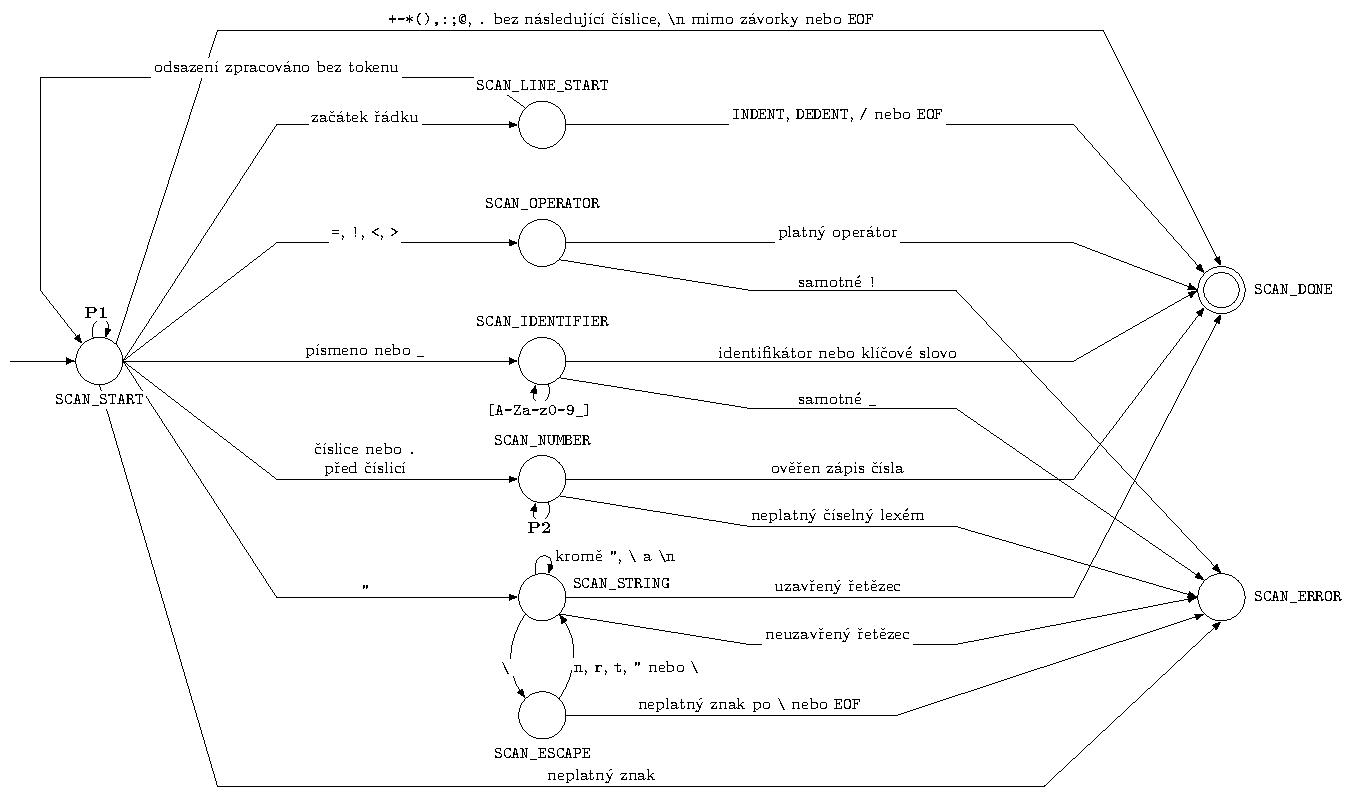
\includegraphics[width=\linewidth, height=118mm, keepaspectratio]{prilohy/automat-diagram.pdf}
\end{center}

\begingroup
\footnotesize

\noindent
\textbf{P1} Mezera, \verb|\t|, \verb|\r|, \verb|\n| uvnitř závorek nebo komentář, který nevyvolá vydání tokenu. \textbf{P2} Číslice nebo některý ze znaků \verb|._eEdD|. \verb|+| nebo \verb|-| jen bezprostředně za \verb|e| nebo \verb|E|.

\smallskip
\noindent
Odsazení si lexer pamatuje na zásobníku, hloubku závorek a blokových komentářů počítá zvlášť. Když ve stavu \texttt{SCAN\_START} narazí na \texttt{/}, kterým nezačíná komentář, rovnou vrátí \texttt{TOK\_SLASH}.
\par
\endgroup

\end{landscape}